\documentclass[12pt, twoside]{article}
\usepackage[francais]{babel}
\usepackage[T1]{fontenc}
\usepackage[latin1]{inputenc}
\usepackage[left=7mm, right=7mm, top=7mm, bottom=7mm]{geometry}
\usepackage{float}
\usepackage{graphicx}
\usepackage{array}
\usepackage{multirow}
\usepackage{amsmath,amssymb,mathrsfs}
\usepackage{soul}
\usepackage{textcomp}
\usepackage{eurosym}
 \usepackage{variations}
\usepackage{tabvar}


\pagestyle{empty}

\begin{document}


\section*{\center{Devoir maison 2}}


\bigskip





\fbox{

\begin{minipage}{18cm}
\textit{Devoir � rendre sur feuille grand format petits
carreaux pour le \textbf{jeudi 4 novembre 2010}.}
\end{minipage}
}

\enskip


 \textit{Remarque: La pr�sentation et la \textbf{r�daction} seront prises en
 compte. }


\enskip


\subsection*{Exercice 1}

\begin{enumerate}
  \item Construire un parall�logramme MATH  de centre S. Placer le point O
  milieu du segment [MA].
  \item Justifier que les droites (OS) et (MH) sont parall�les.
\end{enumerate}


\subsection*{Exercice 2}

\begin{center}
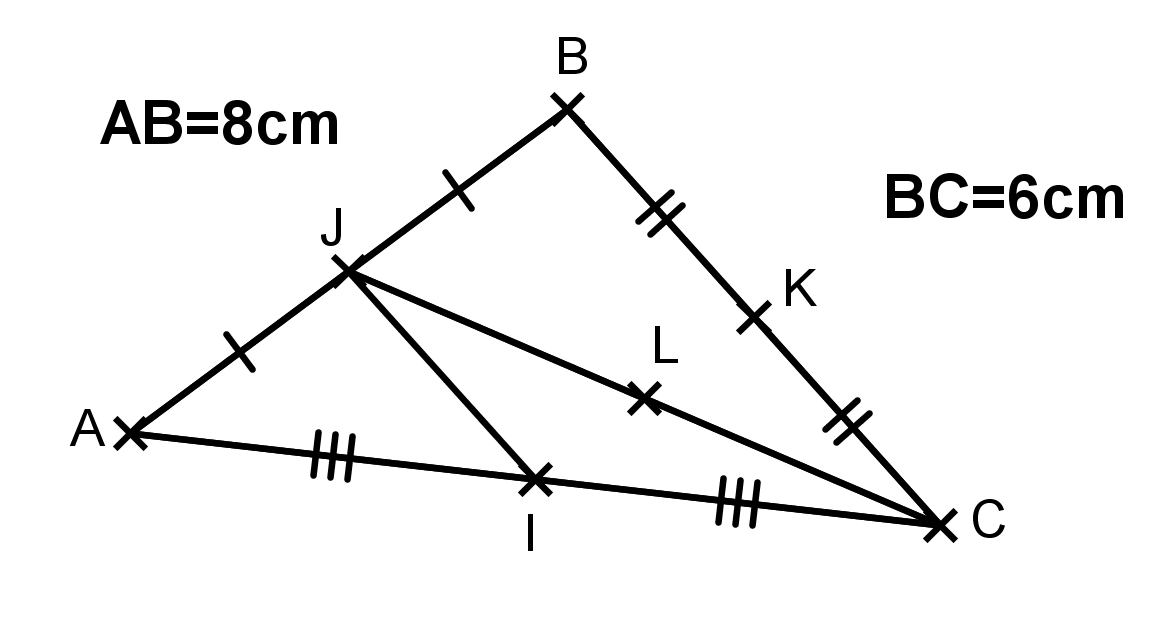
\includegraphics[width=7cm]{images/calcul.png}
\end{center}


\begin{enumerate}
  \item Calculer IJ. Justifier votre r�ponse.
  \item Calculer LK. Justifier votre r�ponse.
\end{enumerate}



\subsection*{Exercice 3}


Dans la figure ci-dessous, P est le milieu de [AB], R est le milieu de [AC], B
est le milieu de [PK] et BC=18cm. 

\begin{tabular}{cc}
\begin{minipage}{13cm}
\begin{enumerate}
  \item Que peut-on dire des droites (PR) et (BC)? Justifier votre r�ponse.
  \item En d�duire que les droites (PR) et (BL) sont parall�les.
  \item D�montrer que L est le milieu de [KR].
  \item Calculer PR. Justifier votre r�ponse.
  \item Calculer BL. Justifier votre r�ponse.
\end{enumerate}
\end{minipage}
&
\begin{minipage}{5cm}
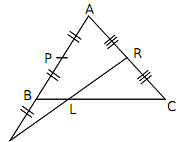
\includegraphics[width=5cm]{images/ex3.png}
\end{minipage}
\end{tabular} 


\subsection*{Exercice 4}


\begin{enumerate}
  \item GAZ est un triangle rectangle en A. Les points F, E et R sont les
  milieux respectifs de [AZ], [GZ] et [GA]. Faire une figure.
  \item Le but de l'exercice est de montrer que le quadrilat�re FERA est un
  rectangle.
  
  \begin{enumerate}
    \item D�montrer que les droites (RE) et (AZ) sont parall�les.
    \item D�montrer que les droites (AG) et (EF) sont parall�les.
    \item Montrer que FERA est un rectangle. Justifer votre r�ponse (on pourra
    commencer par montrer que FERA est un parall�logramme).
\end{enumerate}
\end{enumerate}
\end{document}
